% This file was created by matlab2tikz.
%
%The latest updates can be retrieved from
%  http://www.mathworks.com/matlabcentral/fileexchange/22022-matlab2tikz-matlab2tikz
%where you can also make suggestions and rate matlab2tikz.
%
\documentclass[]{standalone}
\usepackage{amsmath}
\usepackage{graphicx}
\usepackage[pdf]{pstricks}
\usepackage{pgfplots}
\pgfplotsset{compat=newest}
\usepgfplotslibrary{fillbetween}
%% the following commands are needed for some matlab2tikz features
\usetikzlibrary{plotmarks}
\usetikzlibrary{arrows.meta}
\usepgfplotslibrary{patchplots}
\usetikzlibrary{decorations.text}
\usetikzlibrary{shapes.multipart}

\newcommand{\logLogSlopeTriangle}[5]
{
	% #1. Relative offset in x direction.
	% #2. Width in x direction, so xA-xB.
	% #3. Relative offset in y direction.
	% #4. Slope d(y)/d(log10(x)).
	% #5. Plot options.
	
	\pgfplotsextra
	{
		\pgfkeysgetvalue{/pgfplots/xmin}{\xmin}
		\pgfkeysgetvalue{/pgfplots/xmax}{\xmax}
		\pgfkeysgetvalue{/pgfplots/ymin}{\ymin}
		\pgfkeysgetvalue{/pgfplots/ymax}{\ymax}
		
		% Calculate auxilliary quantities, in relative sense.
		\pgfmathsetmacro{\xArel}{#1}
		\pgfmathsetmacro{\yArel}{#3}
		\pgfmathsetmacro{\xBrel}{#1-#2}
		\pgfmathsetmacro{\yBrel}{\yArel}
		\pgfmathsetmacro{\xCrel}{\xArel}
		%\pgfmathsetmacro{\yCrel}{ln(\yC/exp(\ymin))/ln(exp(\ymax)/exp(\ymin))} % REPLACE THIS EXPRESSION WITH AN EXPRESSION INDEPENDENT OF \yC TO PREVENT THE 'DIMENSION TOO LARGE' ERROR.
		
		\pgfmathsetmacro{\lnxB}{\xmin*(1-(#1-#2))+\xmax*(#1-#2)} % in [xmin,xmax].
		\pgfmathsetmacro{\lnxA}{\xmin*(1-#1)+\xmax*#1} % in [xmin,xmax].
		\pgfmathsetmacro{\lnyA}{\ymin*(1-#3)+\ymax*#3} % in [ymin,ymax].
		\pgfmathsetmacro{\lnyC}{\lnyA+#4*(\lnxA-\lnxB)}
		\pgfmathsetmacro{\yCrel}{\lnyC-\ymin)/(\ymax-\ymin)} % THE IMPROVED EXPRESSION WITHOUT 'DIMENSION TOO LARGE' ERROR.
		
		% Define coordinates for \draw. MIND THE 'rel axis cs' as opposed to the 'axis cs'.
		\coordinate (A) at (rel axis cs:\xArel,\yArel);
		\coordinate (B) at (rel axis cs:\xBrel,\yBrel);
		\coordinate (C) at (rel axis cs:\xCrel,\yCrel);
		
		% Draw slope triangle.
		\draw[#5]   (A)-- node[pos=0.5,anchor=north] {1}
		(B)-- 
		(C)-- node[pos=0.5,anchor=west] {#4}
		cycle;
	}
}

\begin{document}

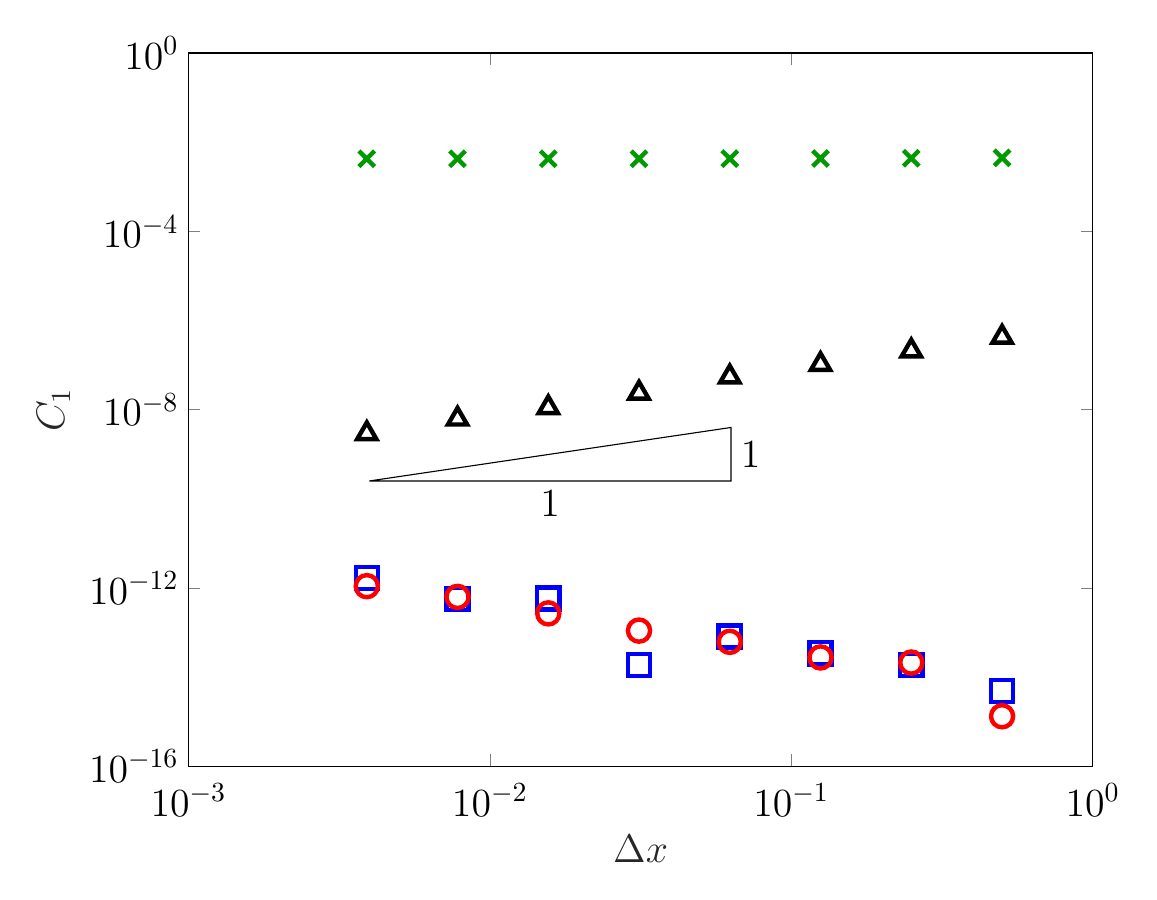
\begin{tikzpicture}
\tikzstyle{every node}=[font=\Large]
\begin{axis}[%
width=4.521in,
height=3.566in,
at={(0.758in,0.481in)},
every axis plot/.append style={ultra thick},
scale only axis,
xmode=log,
xmin=0.001,
xmax=1,
xtick={0.0001,  0.001,   0.01,    0.1,      1,     10},
xminorticks=false,
xlabel style={font=\color{white!15!black}},
xticklabel style = {yshift=-0.1cm},
xlabel={\Large $\Delta x$},
ymode=log,
ymin=1e-16,
ymax=1,
ytick={ 1e-16,  1e-12,  1e-08, 0.0001,      1},
yminorticks=false,
ylabel style={font=\color{white!15!black}},
ylabel={\Large $C_1$},
axis background/.style={fill=white},
legend style={at={(0.03,0.97)}, anchor=north west, legend cell align=left, align=left, draw=white!15!black}
]

\logLogSlopeTriangle{0.6}{0.4}{0.4}{1}{black};

\addplot [color=blue, draw=none, mark=square, mark size=4pt, mark options={solid, blue}]
  table[row sep=crcr]{%
0.500500500500501	4.8457877710462e-15\\
0.250125062531266	1.84838124065807e-14\\
0.125031257814454	3.40975248036528e-14\\
0.0625078134766846	8.16927278416674e-14\\
0.0312519532470779	1.87950490726503e-14\\
0.0156254882965093	5.79330020399846e-13\\
0.00781262207221988	5.678189864958e-13\\
0.00390628051781655	1.65936011952691e-12\\
};
%\addlegendentry{h}

\addplot [color=red, draw=none, mark=o, mark size=4pt, mark options={solid, red}]
  table[row sep=crcr]{%
0.500500500500501	1.32397567221896e-15\\
0.250125062531266	2.11802604225621e-14\\
0.125031257814454	2.7585362156933e-14\\
0.0625078134766846	6.179893706439e-14\\
0.0312519532470779	1.10362142822914e-13\\
0.0156254882965093	2.68861644203969e-13\\
0.00781262207221988	6.29327384942957e-13\\
0.00390628051781655	1.09640876457658e-12\\
};
%\addlegendentry{G}

\addplot [color=black, draw=none, mark=triangle, mark size=4pt, mark options={solid, black}]
  table[row sep=crcr]{%
0.500500500500501	4.22543678106702e-07\\
0.250125062531266	2.09159990347029e-07\\
0.125031257814454	1.03586853596138e-07\\
0.0625078134766846	5.447015874151e-08\\
0.0312519532470779	2.35807541508235e-08\\
0.0156254882965093	1.11043485818812e-08\\
0.00781262207221988	6.17132472686527e-09\\
0.00390628051781655	2.90654630335971e-09\\
};
%\addlegendentry{uh}

\addplot [color=green!60!black, draw=none, mark=x, mark size=4pt, mark options={solid, green!60!black}]
  table[row sep=crcr]{%
0.500500500500501	0.00446569785761301\\
0.250125062531266	0.00436045260042087\\
0.125031257814454	0.00430659009580648\\
0.0625078134766846	0.00427966929615777\\
0.0312519532470779	0.00426622203737353\\
0.0156254882965093	0.00425933971962081\\
0.00781262207221988	0.0042560478776245\\
0.00390628051781655	0.00425440490300424\\
};
%\addlegendentry{H}

\end{axis}
\end{tikzpicture}%

\end{document}